\documentclass[conference]{IEEEtran}
\IEEEoverridecommandlockouts
% The preceding line is only needed to identify funding in the first footnote. If that is unneeded, please comment it out.
\usepackage{cite}
\usepackage{amsmath,amssymb,amsfonts}
\usepackage{algorithmic}
\usepackage{graphicx}
\usepackage{textcomp}
\usepackage{xcolor}
\usepackage{multirow}
\usepackage{hyperref}

\newcommand{\cm}[1]{\textit{{\color{blue}#1}}}
\newcommand{\mr}[1]{\textit{{\color{red}#1}}}

\def\BibTeX{{\rm B\kern-.05em{\sc i\kern-.025em b}\kern-.08em
    T\kern-.1667em\lower.7ex\hbox{E}\kern-.125emX}}
\begin{document}

\title{Towards Reliable Machine Learning Deployments in the Cloud}
% \thanks{Identify applicable funding agency here. If none, delete this.}
\author{\IEEEauthorblockN{1\textsuperscript{st} Charles Meyers}
\IEEEauthorblockA{\textit{Dept. of Computing Science} \\
\textit{Umeå University}\\
Umeå, Sweden \\
cmeyers@cs.umu.se}
\and
\IEEEauthorblockN{2\textsuperscript{nd} Mohammad Reza}
\IEEEauthorblockA{\textit{Dept. of Computing Science} \\
\textit{Umeå University}\\
Umeå, Sweden \\
fake@fake.se}
\and
\IEEEauthorblockN{3\textsuperscript{rd} Tommy Löfstedt}
\IEEEauthorblockA{\textit{Dept. of Computing Science} \\
\textit{Umeå University}\\
Umeå, Sweden \\
tommy@cs.umu.se}
\and
\IEEEauthorblockN{4\textsuperscript{th} Erik Elmroth}
\IEEEauthorblockA{\textit{Dept. of Computing Science} \\
\textit{Umeå University}\\
Umeå, Sweden \\
elmroth@cs.umu.se}
}

\maketitle

\begin{abstract}
Considering the growing prominence of production-level AI and the threat of adversarial attacks that can poison a machine learning model against a certain label, evade classification, or reveal sensitive data about the model and training data to an attacker, adversaries pose fundamental problems to machine learning systems. Prior research has noted the need to extend beyond the normal train-test split paradigm for evaluating models due of the ease with which one can generally find adversarial counterexamples. Additionally, testing model changes likely means deploying the models to a car, medical imaging device, or drone to see how it affects performance, making un-tested changes a public problem. Furthermore, the relationship between model learning rate, batch size, training time, convergence time, and deployment cost is highly complex. So, instead of this train-test split methodology, we propose using accelerated failure time models to measure the effect of hardware choice, batch size, number of epochs, and learning rate by using adversarial attacks to induce failures on a reference model architecture. We evaluate several GPU types and use the Tree Parzen Estimator to maximize model robustness and minimize model run-time simultaneously. In this way, we can evaluate the model and optimize it in a single step, which provides a precise way to not only measure the effect of different hardware deployments but also of the model parameters. Using this technique, we demonstrate that newer, more-powerful hardware does decrease the training time, but with a monetary and power cost that far outpaces the marginal gains in accuracy.
\end{abstract}

\begin{IEEEkeywords}
artificial intelligence, machine learning, adversarial AI, optimization, compliance
\end{IEEEkeywords}


\section{Introduction}
\subsection{Motivations}
% \begin{itemize}
%     % \item \textbf{BIG} Data is the trend
%     % \item Costs are astronomical
%     \item Prevailing regulatory framework is clear about the robustness requirements, documented software changes, and explainable processes.
%     \item Other work relies on unreliable test/train split methodology
%     \item Which means that cars, medical equipment is tested in the wild
% \end{itemize}

Recently, machine learning using neural networks has become a popular way to classify large amounts of data---with applications ranging from medical imaging~\cite{ai_medical_imaging} to aviation~\cite{ai_aviation} and from security~\cite{ai_security,ai_luggage,ai_prison} to self-driving cars~\cite{ai_automotive}. However, neural networks need large amounts of data\cite{desislavov2021compute,bailly2022effects} to train ever-larger model~\cite{desislavov2021compute}, yielding increasingly marginal gains on test-set accuracy~\cite{sun2017revisiting}. Furthermore, popular models like Generative Pre-trained Transformer (GPT)\cite{floridi2020gpt} or ResNet~\cite{resnet} have many millions of parameters, requiring equally large training datasets. Media reports place the cost of training a large language model somewhere between 4 and 63 million dollars~\cite{}, meaning only a few entities in the whole world have the requisite hardware and/or cloud budget to build a competing system. Facebook's large language model, dubbed LLaMA, was placed on the codesharing website, GitHub~\cite{llama}. Immediately, an open-sourced clone was created, which itself spawned hundreds of offshoot projects~\cite{openllama}. The newest version of this open-source large language model (LLM) is able to outperform the commercially available GPT-3.5 model with a fraction of the parameters (13 Billion), small enough to run on a laptop without a graphics processing unit (GPU)~\cite{liu2023goat}. Given the immense cost of deploying modern neural networks, the required number of test samples creates serious questions about the efficacy of the typical train/test split methodology for evaluating the ability of a model to generalize beyond a training set~\cite{meyers} since regulatory standards around safety-critical software applications~\cite{IEC61508,iso26262,aviation_software,safetyframework} clearly define the maximum failure rate to be between $[1e-12, 1e-15]$ depending on the number of lives at risk ~\cite{iso26262}. Collecting, labelling, and testing a new set of data for every software change-as required by law would be prohibitively expensive. Therefore, a new evaluation methodology is required. As such, we propose an evaluation metholodgy, centered around survival analysis, which tests a model against `worst-case' input to verify the efficacy of one of modelling deployment decision over another. Then, we use this method to examine and minimize the deployment cost for a singule model architecture, measuring this in terms of both power and monetary cost. In short, our goal is to answer three questions, 


\subsection{Research Questions}
Our goal is to answer the following three questions:
\begin{itemize}
    \item What is the relationship between latency, robustness, and deployment cost?
    \item What is the cheapest way to guarantee a certain response time and accuracy?
    \item Does better hardware lead to better models?
\end{itemize}

However, before we can answer these questions, we need to model the asymptotic behavior of various architectural choices, develop a method for precisely measuring model performance without resorting to trillions of test samples, and find a metric (or metrics) that will set one model apart from the others with respect to both failure rate and deployment cost. 

\subsection{Contributions}
\begin{itemize}
    \item We confirm previous work about the efficacy of adversarial analysis for model selection.
    \item We measure the power and monetary cost of deploying a model across three different hardware architectures.
    \item We combine survival analysis with adversarial analysis to build accelerated failure models to compare the effect of model parameter choices.
    \item We use a Tree Parzen Estimator to minimize deployment cost while maximizing accuracy.
    \item Show that smaller models running on smaller hardware is far more cost effective, especially in the context of adversarial robustness.
\end{itemize}


\section{Background}
Machine learning pipelines play a crucial role in the development and deployment of robust and accurate models. However, managing complex pipelines across diverse CPU and GPU architectures, ensuring robustness against adversarial attacks, and understanding the relationship between computational cost, model loss, and prediction accuracy remain ongoing challenges. In this paper, we present a comprehensive study on leveraging Kubernetes~\cite{k8s} to manage a complex machine learning pipeline. We explore the robustness of the pipeline under adversarial attacks and examine the impact of computational cost on model performance in both benign and adversarial contexts.

Machine learning applications have witnessed tremendous growth in recent years, addressing a wide range of domains and providing significant advancements in various fields \cite{li_general_2016, croce_reliable_2020, athalye_obfuscated_2018}. As these applications become more sophisticated, the need to efficiently manage the underlying machine learning pipeline arises. The pipeline involves a series of interconnected steps, including data preprocessing, model training, post-processing, and inference. Efficiently orchestrating these steps across diverse CPU and GPU architectures poses significant challenges in terms of scalability, resource allocation, and workload distribution.

To address these challenges, containerization and orchestration technologies have gained prominence in managing complex machine learning pipelines. Kubernetes, a widely adopted container orchestration platform, provides a scalable and flexible environment for deploying, scaling, and managing microservices-based applications. Its ability to handle heterogeneous hardware architectures and workload distribution across clusters makes it an ideal choice for managing the complex computational requirements of machine learning pipelines.

Furthermore, ensuring the robustness of machine learning  models against adversarial attacks has become a critical concern~\cite{adversarialpatch, carlini_towards_2017, croce_reliable_2020, hopskipjump, chakraborty2018adversarial, art2018}. Adversarial attacks aim to exploit vulnerabilities in models by introducing subtle modifications to data submitted to various stages of the ML pipeline, leading to misclassification or otherwise erroneous outputs. Evaluating the robustness of ML models against adversarial attacks is crucial to assess their reliability and performance in real-world scenarios. By subjecting the ML pipeline to carefully crafted adversarial inputs, we can measure its resilience and identify potential vulnerabilities.

Additionally, understanding the relationship between computational cost, model loss, and prediction accuracy is vital for optimizing the pipeline's performance. Balancing computational resources, time constraints, and accuracy requirements is a fundamental consideration in deploying machine learning models in production environments. By analyzing the impact of computational cost on model loss and accuracy metrics, we can gain insights into the trade-offs involved and make informed decisions to optimize the pipeline's efficiency.

In this paper, we present a comprehensive study that combines Kubernetes as the underlying infrastructure for managing a complex ML pipeline across a variety of CPU and GPU architectures. We can investigate the robustness of the pipeline against adversarial attacks and explore the relationship between computational cost, model loss, and  prediction accuracy in both benign and adversarial contexts. Our experiments and analysis provide valuable insights into the trade-offs and considerations when deploying machine learning models under varying computational constraints and adversarial conditions.


For the sake of the reader, we provide a section for definitions and requisite background information below.

\subsection{Cloud Architectures}
A \textbf{microservice} is the smallest component of a `cloud-native' software stack. In the context of machine learning, that might be a tool for either training, inference, pre-processing, sampling, or any other arbitrarily small part of the data pipeline. A microservice \textbf{mesh} is a network infrastructure or architectural pattern that provides a unified and scalable approach to managing communication between microservices in a distributed system. It serves as a dedicated layer that abstracts away the complexity of service-to-service communication, enabling efficient and reliable interactions among these services. A microservice mesh typically consists of a set of interconnected components or proxies deployed alongside the microservices within the system. These components facilitate various capabilities and functionalities essential for managing the communication between microservices. Kubernetes has become one of the largest open source projects on the code-sharing website Github \cite{k8s-size}, which provides a framework for managing, monitoring, and networking a self-scaling set of tools across arbitrary software and hardware architectures.

\subsection{Machine Learning Pipelines}
Machine Learning pipelines are often long-running and complex software tool-chains with many tunable hyperparameters. Managing, tracking, and controlling for various parameters is non trivial, but many management tools are available~\cite{dvc, hydra, k8s}. In general, a dataset is split into \textbf{training} and \textbf{test} sets. The training set is then used to determine the best configuration of a given model architecture on a given hardware architecture with the expectation that it will generalize both on the withheld test set and on new data generated by users via application programming interface (API) calls. To verify the training process, the test set validated against the \textit{inference} configuration of a model which may run on different hardware than the \textbf{training} configuration to reduce cost, latency, or power consumption. 

\subsection{Classifiers}

A classifier with model parameters, $\theta$, $K(x; \theta)$, drawn from a set of all possible hyper-parameters, $\Theta$, seeks to minimize\footnote{This can also be formulated as a maximization function without loss of generality.} an \textbf{objective} (or \textbf{loss}) \textbf{function} $L(y, \hat{y})$ for some samples, $x$, some true labels $y$, and some model output, $K(x)$, such that the optimal loss value, $L^*$ is:
\[
L^*(y, K(x, \theta)) = \mathrm{argmin}_{\theta \in \Theta} y - K(x, \theta).
\]
From here, we can find the optimal configuration of the classifier by selecting the one that minimizes loss. In the case of neural-networks, however, this is non-trivial as the number of tunable parameters is often measured in the millions. Instead of finding an analytical solution to this equation, we often rely on \textbf{stochastic gradient descent}, which iteratively shuffles the data before adjusting the model parameters, $\theta$, in the direction that minimizes the loss, $-\nabla L(y, K(x, \theta))$, after some number of \textbf{epochs} (iterative random sampling of the data), $m$, such that:
\begin{equation}
\theta_{m+1} := \theta_{m} - \eta \nabla_x L(y, K(x, \theta_m))
\label{eq:sgd}
\end{equation}
where $\eta$ is a \textbf{learning rate} that is tuned to the particular model. 

\subsection{Learning Rate Selection}
\label{learning_rate}
\cm{TODO}
\begin{itemize}
    \item Much work has gone into this~\cite{}.
    \item A good learning rate will give us training times that are linear w.r.t sample size ~\cite{}
    \item Will depend on the batch size and number of epochs (define epochs) ~\cite{}
    \item The best batch size will depend on the memory bandwidth of the GPU~\cite{}
    \item That bandwidth is not guaranteed in on-demand cloud environments~\cite{}
    \item Hardware is charged by the hour, so minimizing training/inference times will reduce the costs of deployment.
\end{itemize}

\subsection{Adversarial Attacks}
\label{attacks}
In the context of machine learning, an adversarial attack refers to deliberate and malicious attempts to manipulate or exploit machine learning models. Adversarial attacks are designed to deceive or mislead the model's behavior by introducing carefully crafted input data that can cause the model to make incorrect predictions or produce undesired outputs. That is, a successful attack is one in which the model outputs on unperturbed data $\hat{y}$ are not the same as the model outputs on perturbed data, $x'$. That is \textbf{adversarial success} or \textbf{accelerated failure} is one in which:
\begin{equation}
\hat{y} \neq y^* = K(x', \theta)
\label{eq:adv_success}
\end{equation}
Additionally, we can measure the accuracy of the model when tasked with these adversarial samples, giving us a metric called \textbf{adversarial accurracy}. The goal of an adversarial attack is often to exploit vulnerabilities in the model's decision-making process or to probe its weaknesses. These attacks can occur during various stages of the machine learning pipeline, including during training, inference, or deployment. 

\cm{This itemize section could be cut and reduced to a couple sentences.}
\begin{itemize}
    \item Evasion Attacks: These attacks aim to manipulate input data during the inference phase to deceive the model into misclassifying or ignoring certain inputs. Attackers carefully craft perturbations or modify the input features to mislead the model while still appearing similar to the original input \cite{biggio_evasion_2013, carlini_towards_2017, adversarialpatch, pixelattack, hopskipjump}.
    \item Poisoning Attacks: In poisoning attacks, the attacker intentionally injects malicious or manipulated training samples into the training dataset. The goal is to influence the model's behavior during training so that it learns to make incorrect predictions or exhibit unwanted behaviors when presented with specific inputs \cite{biggio_poisoning_2013, saha2020hidden}.
    \item Inference Attacks: These attacks exploit the model's output or responses to obtain sensitive information about the training data or other confidential details. By observing the model's predictions or confidence scores for carefully crafted inputs, attackers can extract information that should ideally be kept private \cite{chakraborty_adversarial_2018, orekondy2019knockoff}.
    \item Model Inversion Attacks: Model inversion attacks aim to infer sensitive information about the training data or proprietary model by exploiting the model's outputs. Attackers utilize the model's responses to iteratively reconstruct or approximate training examples that are similar to the ones used during training \cite{chakraborty_adversarial_2018, choquette2021label, li2021membership}.
\end{itemize}
One attack designed to induce failures as quickly as possible~\cite{fgm} works by applying noise to a set of samples, $x$, to generate adversarial examples, $x'$, such that:

\begin{equation}
x' = x + \eta \mathrm{~sgn~}(\nabla_x L(y, K(x, \theta))).
\label{eq:fgm}
\end{equation}
In essence, this is stochastic gradient \textit{ascent}, the opposite process from model training (stochastic gradient \textit{descent}).

\subsection{Adversarial Analysis}

In the case of safety- or security-critical domains, considering the worst-case scenario is routine~\cite{}. Whether we discuss automotive safety~\cite{}, crytographic systems~\cite{}, or healthcare malpractice~\cite{}, a component, algorithm, or system is considered broken if the \textbf{failure rate} exceeds certain statistical thresholds. An order of magnitude more automotive accidents, security breaches, or deaths due to medical negligence would be unacceptable and, as such, these standards are non-negotiable. However, this would mean testing somewhere around $(10^6, 10^9)$ samples to justify every model change. This is just not computationally feasible. Instead, we can use adversarial failure analysis to improve the precision of our measurements while only using a small set of test-data.

\subsubsection{Accuracy}
The failure rate, denoted by $h$, refers to the percentage or proportion of examples that cause the targeted machine learning model to misclassify or produce incorrect outputs \cite{meyers}. It measures the vulnerability or susceptibility of the model to noise-induced failures. A higher failure rate indicates a higher rate of misclassifications or incorrect predictions, signifying a weaker model in terms of \textbf{robustness} against noise-induced failures. Throughout, we use the terminology \textbf{benign accuracy} to refer to the performance on the test set using unperturbed data. The benign accuracy is defined as
\begin{equation}
 \mathrm{Accuracy} = 1 - \frac{\mathrm{False~Classifications}}{\mathrm{Total~Classifciations}}
\label{eq:acc}
\end{equation}
which is generally assumed to indicate the rate of failures in real-world data drawn from the same distribution as the test data \cite{}. However, the normal test/train split methodology consistently overestimates the model's performance in the presence of adversarial noise~\cite{croce_reliable_2020}. Additionally, it has been shown that generating adversarial counter examples that dispute this train/test split analysis is trivial~\cite{biggio_evasion_2013,carlini_towards_2017,adversarialpatch,pixelattack,hopskipjump,biggio_poisoning_2013,chakraborty_adversarial_2018,dohmatob_generalized_2019,meyers}. In addition, this method ignores the run-time cost of a given architectural decision, caring only for marginal accuracy gains on benchmark data~\cite{}. Instead, we can measure the computational feasibility of finding noisy counterexamples close to the original samples, such that 
$$
y\neq\hat{y}\mathrm{~s.t.~}\| x' - x \| \leq \varepsilon \leq \varepsilon_{max}
$$ 

where $\| \cdot \|$ represents some norm or pseudo-norm and $\varepsilon$ is some specified distance threshold bound by some distance, $\varepsilon_{max}$.


\subsubsection{Failure Rate}
 To encompass the cost of a particular model or attack, we can think of the failure rate as a function of time (\textit{e.g.} training time, inference time, attack generation time, etc.) and some covariates (\textit{e.g.} noise distance, model size, hardware resources) such that:
\[
h(t; \theta) :=  \frac{\mathbb{P}(\textrm{False~Classification})}{\Delta t}
\]
where $\mathbb{P}$ is a probability and $\Delta t$ is a time interval. To get a more precise and reliable estimate of a model's failure characteristics, we can use accelerated failure time models that model the \textbf{survival time}, $S(t)$, as a function of the samples, $x$, the labels, $y$, and some set of covariates, $\theta$ such that:
\[
S(t; x,y, \theta) := 1 - \int_{t=0}^{\infty} h(t;\theta) d \theta
\]

\subsection{AFR models}
\label{afr}
Accelerated failure rate models are statistical models used to analyze multivariate effects on the observed failure rate to predict the expected survival time ($\mathbb{E}[S(t; x,y, \theta)]$) across a wide variety of circumstances~\cite{aft_models,kleinbaum1996survival}. However, this requires a choice in modelling distribution for $S$. We tested Log-Logistic, Log-Normal, and Weibull distributions, relying on Akaike Information Criterion (AIC), Bayesian Information Criteria (BIC), and Concordance to choose the best-fit, following the best-practices of other research~\cite{aft_models}.  This analysis allows us to test the model under extreme perturbations, revealing not only the accuracy under ideal test scenarios, but to see the model's performance in the presence of noise that's designed to be adversarial. However, we still have to find optimal configurations for both the attack and defence, which often rely on parameters drawn from continuous or infinite spaces. In order to minimize the cost of evaluation, we must be clever about how we search.

\subsection{Pareto Set}
\cm{This section could probably be cut without too much lost.}
In security analysis, it is customary in security analysis to imagine a best-case scenario for both the defender and the attacker~\cite{}. A subset of examples that maximize one or more objective criteria is called the \textbf{pareto front}~\cite{zitzler2008quality}. It has been shown that we can find an $\varepsilon$-approximation of this front $\mathcal{P}$ in $d$ dimensions using $(1/ \varepsilon)^d$ queries ~\cite{legriel2010approximating}. Table~\ref{tab:pareto} shows the required number of queries to get estimates within the $\varepsilon$-sphere of the true Pareto front. As we can see, it is critical to minimize the dimensionality of our search. So instead of optimizing for latency, training time, cost, accuracy, and adversarial success rate independently, we introduce several metrics in the next section.


% Please add the following required packages to your document preamble:
% \usepackage{multirow}
% Please add the following required packages to your document preamble:
% 
\begin{table}[h!]
\begin{tabular}{cl|llll|}
\cline{3-6}
                                           &   & \multicolumn{4}{c|}{$\varepsilon$}            \\ \cline{3-6} 
                                           &   & .1     & .05          & .01    & .001      \\ \hline
\multicolumn{1}{|c|}{\multirow{3}{*}{$d$}} & 1 & 10     & 20           & 100    & 1000      \\
\multicolumn{1}{|c|}{}                     & 2 & 100    & 400          & $10^4$ & $10^6$    \\
\multicolumn{1}{|c|}{}                     & 4 & $10^4$ & $1.6 * 10^5$ & $10^9$ & $10^{12}$ \\ \hline
\end{tabular}
\caption{This table shows the number of queries required to $\varepsilon-$ approximate the Pareto front, $\mathcal{P}$, in $d$ dimensions.}
\label{tab:pareto}
\end{table}


\subsection{Optimization}

Because of the relatively small run-time requirements of this approach (when compared to testing against massive in-distribution test sets), this method could, for example, act as a unit test in machine learning applications rather than relying on full-system integration tests to evaluate changes to a single model, signal processing technique, data storage format, or API access mechanism. It could also be used to highlight error-prone classes or other subsets of data to reduce error or create synthetic samples. Furthermore, by isolating changes and testing them as quickly as possible, it's much easier to parse cause and effect when compared to full-system integration tests that could include many changes from many different development teams and require live and potentially dangerous systems (like cars or MRI machines) to effectively test. To further increase development velocity, we can use these models to quantify the marginal risk associated with each change, as dictated by the ISO 26262 standard \cite{iso26262}. However, hyper-parameters are often drawn from continuous and infinite spaces, so it's impossible to exhaustively evaluate the search space. Additionally, the goals of test-set accuracy and adversarial accuracy are often at odds, meaning that a proper search would keep this dual-objective in mind. Luckily, the field of multi-objective search is well researched and analyze the run-time requirements for several popular choices below, each of which will be useful for different types of search spaces. We chose the Tree-structure Parzen Estimator (TPE) because of it's ability to work on mini-batches~\cite{}, in distributed settings~\cite{}, and while optimizing multiple objectives~\cite{} in a feasible number of trials ~\cite{}. 




\section{Metrics}

We withheld 100 examples from both the test and train sets as the initial values for adversarial examples, which gives us two significant figures for this measurement. In addition, we measured the model training time ($t_{t}$), the model inference time or latency ($t_{i}$), the cost per hour for a particular hardware ($C$), and the power consumption ($P$) of each tested model and attack, as well as the benign and adversarial accuracies (see: Secs.~\ref{eq:acc} and ~\ref{eq:adv_success}).

\subsection{Accuracy}
We measured both the benign accuracy and the adversarial accuracy, which reflect the normal test-set accuracy and the test-set accuracy in the presence of additive noise in the direction that maximizes loss.

% \subsection{Benign Success}
% A \textit{success} can be thought of in both the adversarial and benign context, which are denoted with the subscripts $ben.,adv.$ throughout this work. Typically this is measured via the train/test methodology in which some subset of a benchmark dataset. However, this method has repeatedly shown itself to be an inadequate measure of real-world model performance, and is, at best, an optimistic best-case measure of the failure rate~\cite{croce_reliable_2020}. The benign success ratio is usually measured via the train/test split methodology mentioned in typical in the literature. 

% \subsection{Adversarial Success}
% A successful adversary, however, is one that is able to change the model's output from one class to another. For the benign case, we measure the test set accuracy as our success metric. However, we m

% Furthermore, the computational difficulty of this task is often related to secondary optimization criteria~\cite{}, with a baseline of at least NP-Hard~\cite{madry2017towards}. Since many of the attacks have more success after a number of iterations\cite{fgm,deepfool,carlini_towards_2017,madry2017towards,hopskipjump}, it is appropriate to think about their success in terms of time.



\subsection{Training Time}
The training time, $T_t$, is the time it takes to evaluate $n$ samples for $m$ epochs such that the training time per sample per epoch $t_t$ is.
$$
T_t := t_t\cdot n\cdot m
$$

\subsection{Latency}
Latency is the time it takes to respond to a query. We assume that latency per sample is:
$$
T_i  := t_i \cdot n 
$$
which will be driven by the memory bandwidth (measured in bits/second) of a given cpu- or gpu-\cite{} and the size\cite{} and complexity\cite{} of a given neural network architecture.

\subsection{Attack Generation Time}
A successful attack is one that induces failure in a model. That is, the expected survival time, $\mathbb{E}[S(t;x,y,\theta)]$, can be thought of as the time it takes for an attacker to induce a change in the model output. We approximate this for each attack/defence configuration by taking the total attack time, $T_a$, for $n$ samples, $i$ iterations, and attack time per sample, $t_a$:

$$
T_a := t_i \cdot n \cdot i 
$$



\subsection{Cost}
Furthermore, we can think of cost of deployment at two scales. Firstly, we consider the cloud-rental scale, where a small-business might test and deploy a model, using GCP compute costs as a measure of total cost. However, at a certain scale, (\textit{e.g.} for deploying a self-driving car) it's more appropriate to talk about cost in terms of power. Finally, we define best-case and worst-case success metrics that give us an efficient way to minimize the latency, cost of deployment, and 

\subsubsection{Hardware}
This value, measured in United States Dollars per hour, will indicate the operating cost of a given model. To calculate this, we used the price per hour from each of cloud service pricing page~\footnote{ Google Cloud prices for P100 and V100 obtained \href{https://cloud.google.com/compute/gpus-pricing}{here.} } ~\footnote{Google Cloud prices for L4 obtained  \href{https://cloud.google.com/compute/vm-instance-pricing#accelerator-optimized}{here.}} and calculated the cost of training ($C_{t}$) and the ($C_{i}$) from the cost of hardware ($C_{h}$), the training time ($T_{t}$) and the inference time ($T_{i}$) such that the cost of training a model is
$$
    C_t = C_h \cdot T_t
    \label{eq:cost_training}
$$
the cost of model inference time is
$$
    C_i = C_h \cdot T_i,
    \label{eq:cost_inference}
$$
and the cost of an attack is:
$$
    C_a = C_h \cdot  T_a.
    \label{eq:cost_attack}
$$

\subsubsection{Power}
The power consumption for a particular piece of hardware ($P_h$), measured in Watts (Joules per second), can be thought of similarly such that the total power consumption of model training is
$$
    P_t = P_h \cdot T_t,
    \label{eq:power_training}
$$
the power consumption during model inference is:
$$
    P_i = P_h \cdot T_i
    \label{eq:power_inference}
$$
and the power consumption during attack generation is:
$$
    P_a = P_h \cdot T_a
    \label{eq:power_attack}
$$

\subsection{Survival Time}
Correspondingly, we can talk about the expected survival time under optimistic, $S_{ben.}$ as well as under adverse (accelerated failure rate distribution), $S_{adv.}$. If we assume that the distribution of failures is uniform with respect to latency, a
$$
S_{ben.} := S(t_i; x, y, \theta) \mathrm{~s.t.~} \varepsilon = 0
$$
and
$$
S_{adv.} :=  S(t_i; x, y, \theta) \mathrm{~s.t.~} 0 < \varepsilon \leq \varepsilon_{max}
$$
\subsection{Relative Cost to an Attacker}
In security analysis, it's routine to think in optimistic terms for both the attacker and defender. As such, we center our analysis on the Fast Gradient Method~\cite{fgm} (see: Eq.~\ref{eq:fgm}) which adds noise of a specified magnitude to some samples in the direction that maximizes loss. If the cost to a model builder ($C_t$) is much larger than the attacker ($C_a$), then it's clear that a configuration. 

% $$
% \frac{\mathrm{Successful~Queries}}{\$} = \frac{\mathrm{Accuracy}\cdot n}{T_i} = 
% $$


\section{Methods}
\subsection{Cloud Platform and Hardware}
To conduct the experiments and have access to different types of hard, we utilized Google Cloud Platform (GCP). Six virtual machines running Container Optimized Operating System provided by GCP constitute our testbed. Using Google Kubernetes Engine 1.27.3 and Containerd 1.7.0,  we created a cluster that comprises of six worker nodes. Three worker nodes were responsible for running the monitoring platform such as Prometheus 2.47.2 and Grafana 10.2.0. These nodes were of the 'e2-medium' instance type provided by Google Cloud Platform. In total, we used three different GPU based on their availability. For both, P100 and V100 GPUs, we used 'n1-standard-2' type for the nodes and for L4  we used 'g2-standard-4' node.
To assess the energy consumption of the experiments deployed on a GKE, we employed Kubernetes Efficient Power Level Exporter (KEPLER) as our measurement tool~\cite{amaral2023kepler}. This approach enables us to gather energy consumption data on granular level as it runs in Kubernetes cluster and capable of collecting energy consumption of Kubernetes components. In essence, KEPLER uses extended Berkley Packet Filter (eBPF) to probe energy-related system stats and exports them as Prometheus metrics. eBPF can be described as a lightweight and sandboxed virtual machine (VM) in kernel space. eBPF programs are invoked by the kernel when certain events, called hooks, occur. Examples of such hooks include system calls or network events. These processes enable deep analysis and full control over different events with low overhead~\cite{sedghpour@ebpf}. A diagram of the cloud architecture can be found in Fig.~\ref{fig:architecture}. Finally, to meet our goal of developing a cost-effective model evaluation technique, we restricted all of our experiments to a single one-thousand United States dollar research grant from Google. 

\begin{figure*}
    \centering
    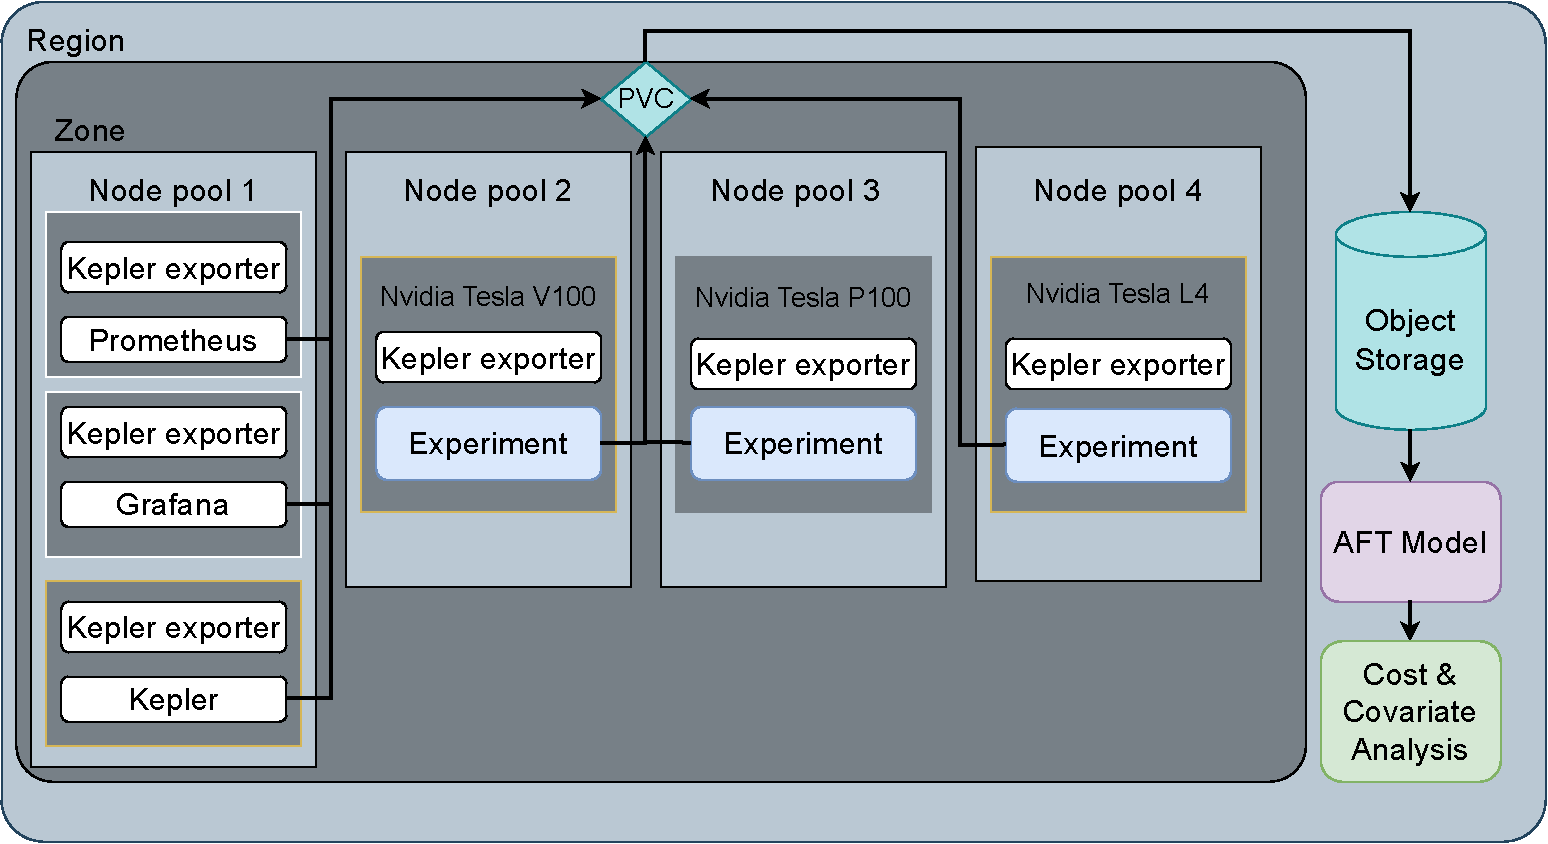
\includegraphics[width=\textwidth]{plots/architecture.pdf}
    \caption{Cloud Architecture Diagram}
    \label{fig:architecture}
\end{figure*}

For each hardware configuration and dataset, we ran one thousand trials, a number that should converge to a pareto-optimal result~\cite{} for the TPE algorithm, within some expected error bounds (see: Tab.~\ref{tab:pareto}). We used three optimization criteria-- benign accuracy, training time, and adversarial accuracy seeking to maximize both benign and adversarial accuracy while minimizing training time (and therefore deployment cost). We selected a set of parameters as per the TPE algorithm and trained on 80\% of the samples. Of the remaining samples, 100 were withheld to be attacked and used to evaluate the adversarial accuracy. Fig.~\ref{fig:experiments} illustrates this methodology. For each dataset, we tested this on ten random splits of the data. 

\begin{figure}
    \centering
    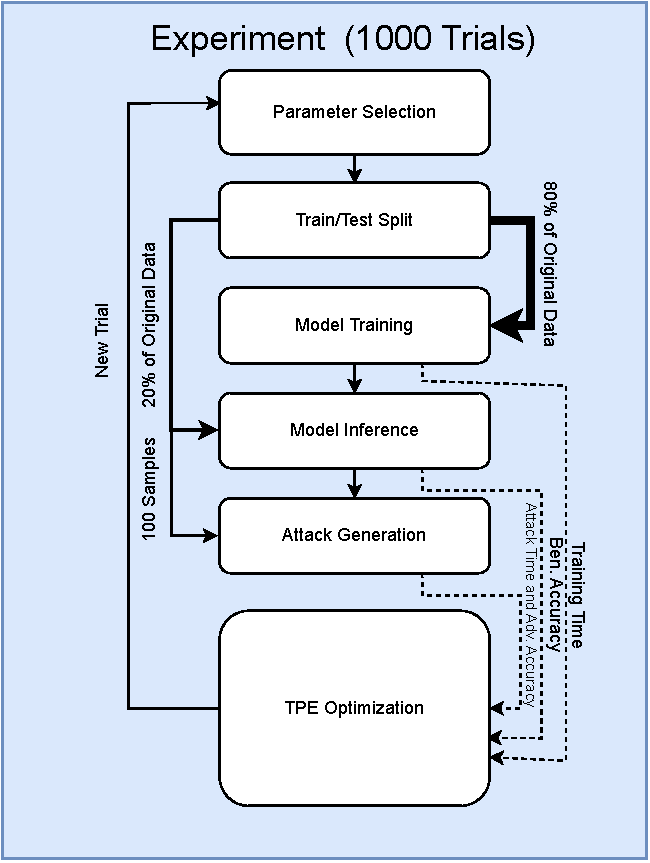
\includegraphics[width=.45\textwidth]{plots/experiment.pdf}
    \caption{Experimental Pipeline Diagram}
    \label{fig:experiments}
\end{figure}


\subsection{Datasets}
For our experiments, we evaluated the MNIST~\cite{mnist}, CIFAR10\cite{cifar}, and CIFAR100\cite{cifar} datasets, chosen primarily for their standardized use in adversarial analysis ~\cite{madry2017towards,croce_reliable_2020,carlini_towards_2017,deepfool} and decades of experimental results. By modern standards (billions of parameters), these models are quite small (tens of thousands of samples), but our goal is not to rival the accuracy of industy leaders, but to develop a method that is practical for everyone else to use.
Before training, we centered and scaled the data so that the attack distance would be analogous for all tested datasets. Furthermore, to reduce the complexities of system overhead, distributed or federated training, and the effect of shared cloud environments, we restricted ourselves to datasets that are small enough to reside entirely within GPU memory with the model, since the disk read speed in cloud environments is incredibly variable.

\subsection{Models}
We restricted ourselves to a single model for our evaluations. Primarily, this was done to meet the budgetary constraints since evaluating more models would mean evaluating fewer pieces of hardware. As discussed in Sec.~\ref{learning_rate}, the relationship between hardware specifications, model-size, data distribution, the optimal learning rate, the optimal batch size, and the optimal number of epochs is highly complex and hard to predict. So, we sampled learning rates $\in [1e-6, 1]$, batch sizes $\in [1, 1e5]$, and epochs $\in [1,50]$ for MNIST and CIFAR10 on the P100 and V100. For Cifar100, we increased the range of the tested epochs to be $\in [1, 100]$. To evaluate the efficacy of different bit-depths on the L4 hardware, we used the Feature Squeezing defence~\cite{feature_squeezing} provided by IBM's adversarial robustness toolbox~\cite{art2018}.

\subsection{Attacks}
Since the goal in this paper is to evaluate how hardware and deployment cost affect adversarial robustness, we focused on evasion attacks since they induce failures by adding noise to the data. Prior research ~\cite{meyers} has shown that the Fast Gradient method (see: Eq.~\ref{eq:fgm}) is consistently the most effective at inducing a large number of failures in a small amount of time. To evaluate the effect of noise on our samples, we varied $\varepsilon \in [0, 1]$.


\subsection{GPU Configurations}
We tested several hardware configurations, which have various hourly costs, peak power demands, and theoretical memory bandwidths. We tested three Nvidia cards-- the V100, the P100, and L4. The V100 was chosen as a baseline since it's allegedly the hardware behind large LLMs like GPT~\cite{}. The P100 architecture comes from the same line of server-grade training GPUs, but from an older generation. The L4, however, is advertised as a machine built for inference--not training, relying on a smaller number of bits per tensor core. Consequently, the number of operations per second is dependent on the bit depth of the data and the model weights, with the peak numbers outlined in Tab.~\ref{tab:hardware} referring to 8-bit inputs.
\begin{table}[h]
\begin{tabular}{lllll}
\hline
                        & V100   & P100   & L4    &  \\ \hline
Cost (USD/hour)          & 2.55 & 1.60 & .81 &  \\
Power (Watts)           & 250    & 250    & 72    &  \\
Memory Bandwidth (GB/s) & 900    & 732    & 300   &  \\ \hline
\label{tab:hardware}
\end{tabular}
\caption{Hardware specifications for tested GPUs. All specifications were retrieved from the Nvidia website at the following links: 
\href{https://images.nvidia.com/content/technologies/volta/pdf/volta-v100-datasheet-update-us-1165301-r5.pdf}{V100 Datasheet},
\href{https://images.nvidia.com/content/tesla/pdf/nvidia-tesla-p100-PCIe-datasheet.pdf}{P100 Datasheet}, and
\href{https://nvdam.widen.net/s/rvq98gbwsw/l4-datasheet-2595652}{L4 Datasheet}. Prices were retrieved from Google Cloud Platform for the \texttt{europe-west4} region on 3 December 2023 at \href{https://cloud.google.com/pricing/list}{this link.}
}
\end{table}

\section{Results}
\cm{Here are most of the results. I'm still playing with how to 1. combine the hardware into a single model per dataset or 2. visualize 9 different combinations in a tiny space. I'd very much like to show the partial effects plots as I did before with the layers in the NEURIPS paper.}

\subsection{Accuracy and Robustness}
Marginal gains in accuracy for faster hardware, but no significant change in survival time.
\begin{figure*}
    \centering
    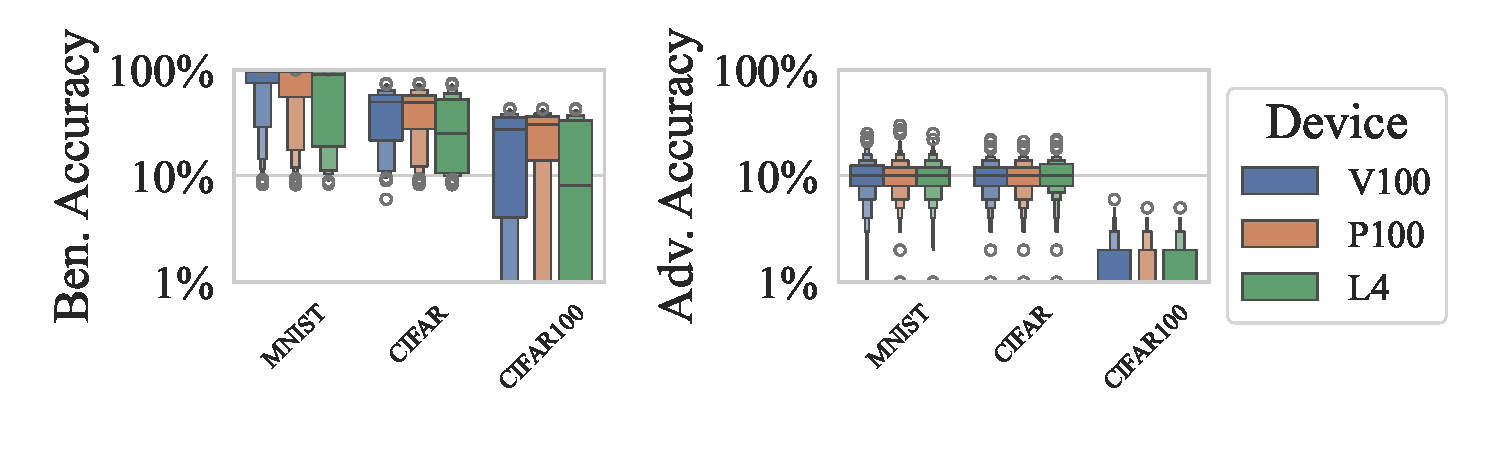
\includegraphics[width=\textwidth]{plots/combined/acc.pdf}
    \caption{Ben. and Adv. Accuracy Across Datasets and Hardware}
    \label{fig:acc}
\end{figure*}

\subsection{Time}
Corresponds roughly to what we would expect from the peak GPU bandwidth numbers in Tab.~\ref{tab:hardware}.

Slower hardware is marginally slower. Results would be undetectable for a user with a reasonably small query.


\begin{figure*}
    \centering
    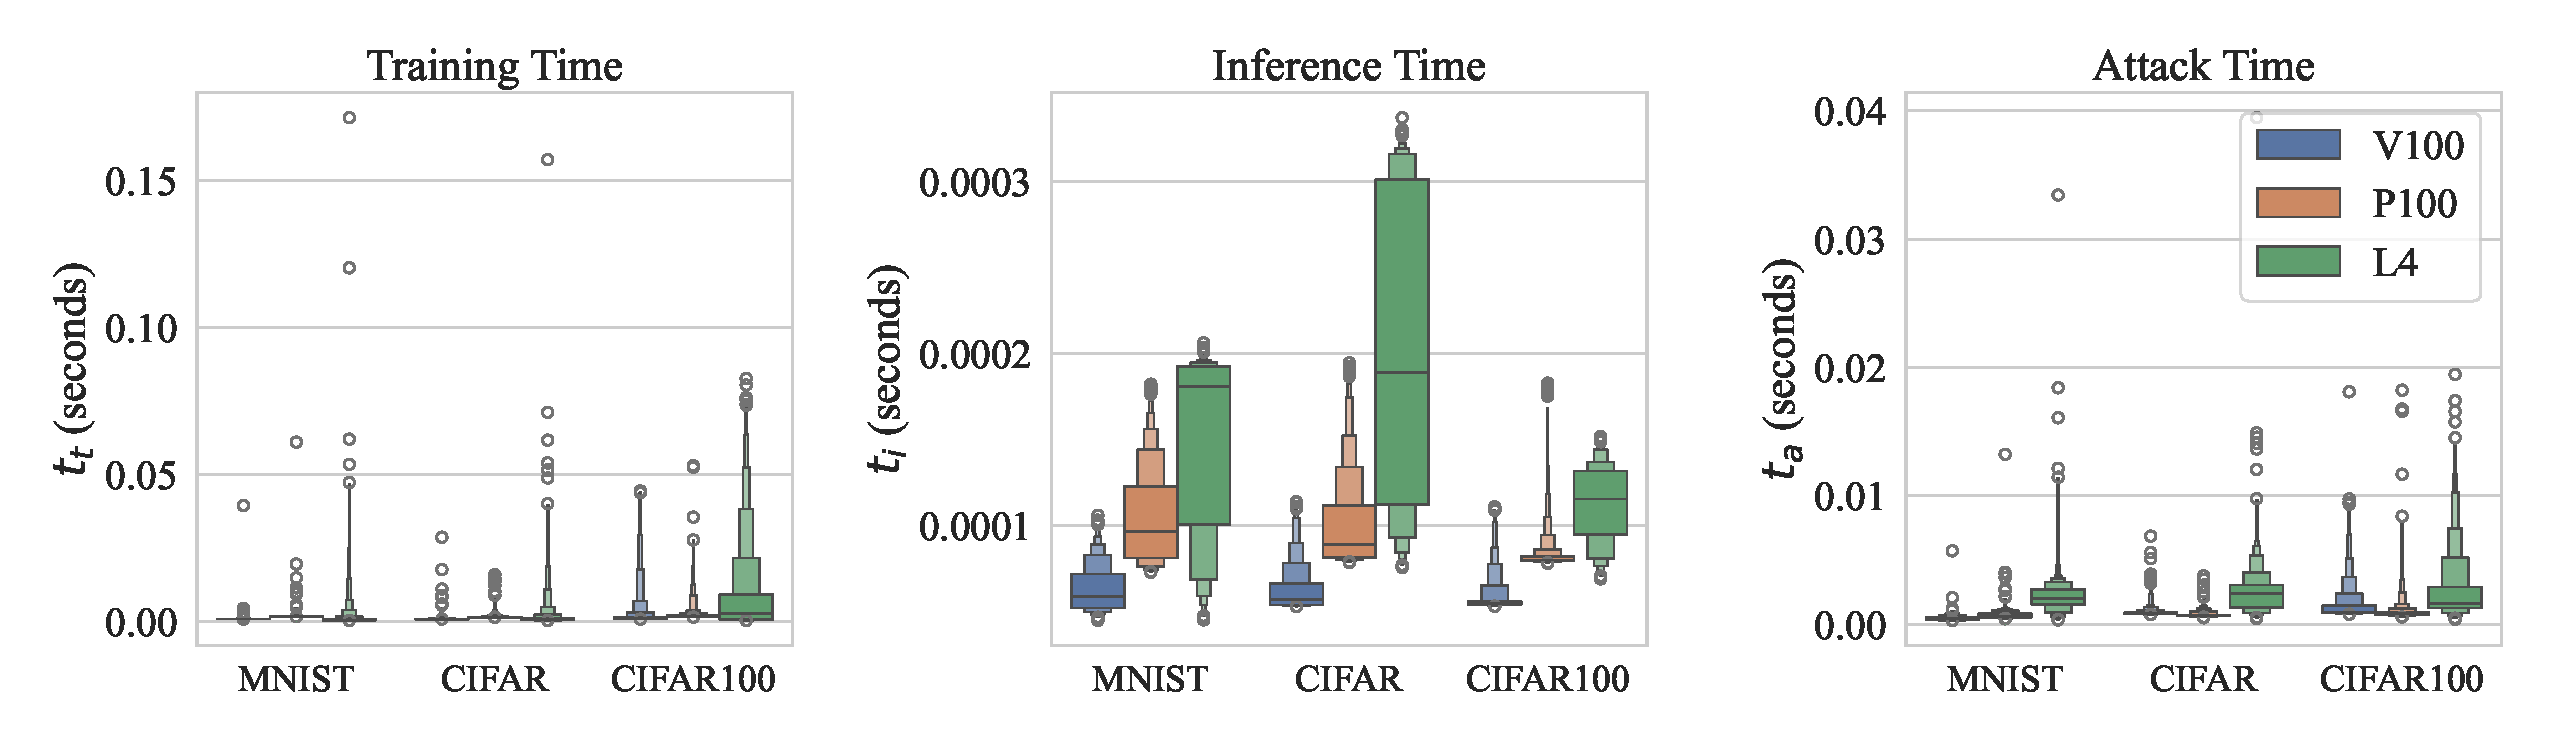
\includegraphics[width=\textwidth]{plots/combined/time.pdf}
    \caption{Training, Prediction, and Attack times across datasets and hardware.}
    \label{fig:time}
\end{figure*}





\subsection{Monetary Cost}


\begin{figure*}
    \centering
    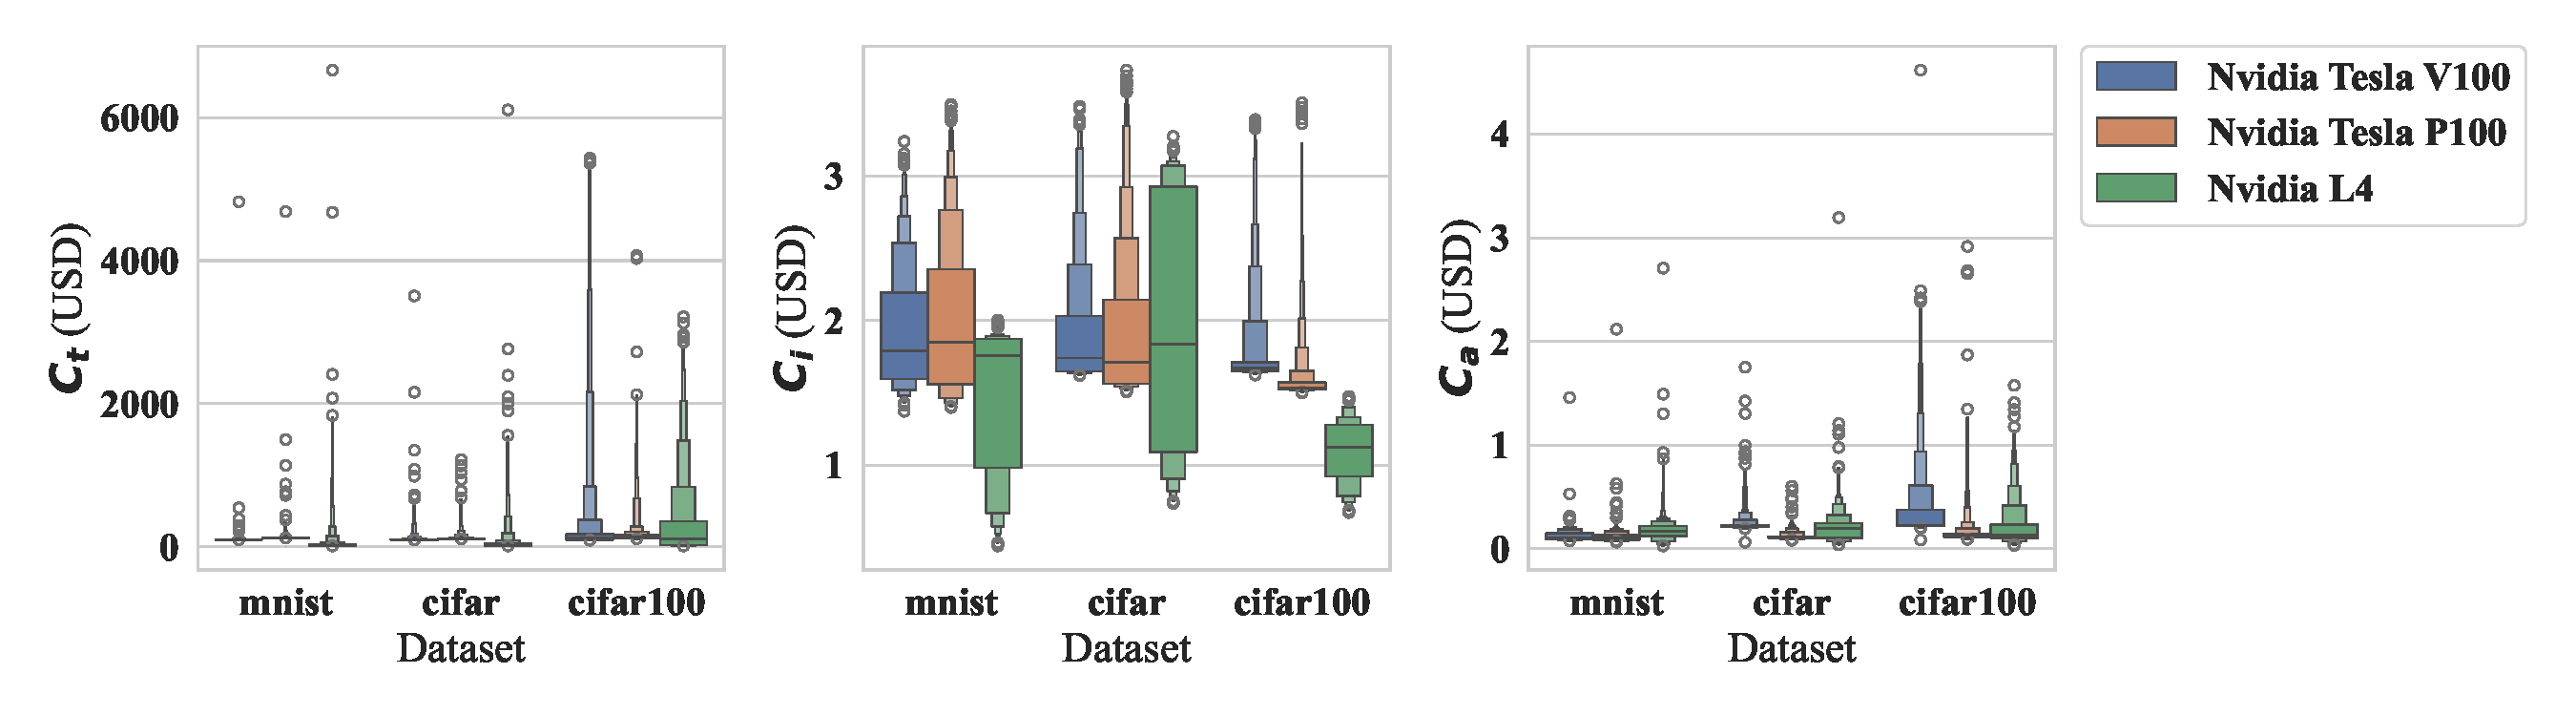
\includegraphics[width=\textwidth]{plots/combined/cost.pdf}
    \caption{Training, Prediction, and Attack Power Consumption Across Datasets and Hardware}
    \label{fig:time}
\end{figure*}
Smaller hardware is significantly cheaper (roughly half the cost to train vs. the best hardware).

\subsection{Power}
\begin{figure*}
    \centering
    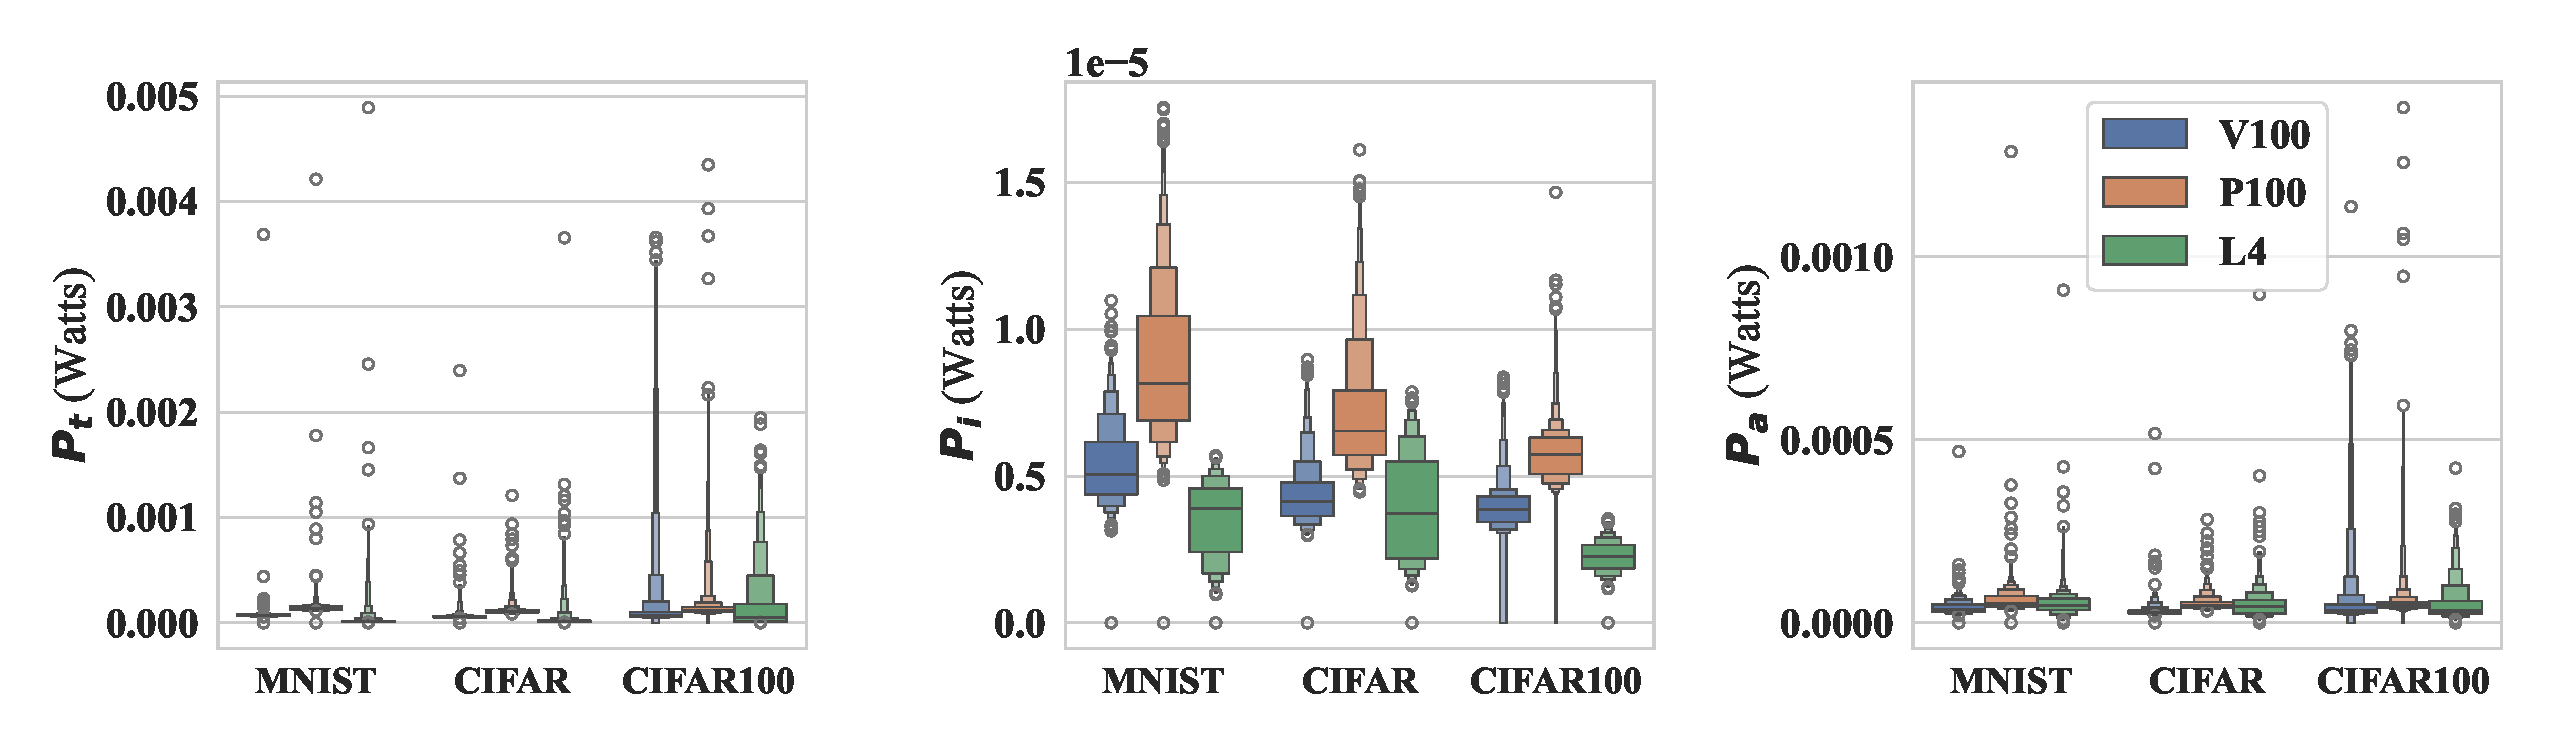
\includegraphics[width=\textwidth]{plots/combined/power.pdf}
    \caption{Training, Prediction, and Attack Power Consumption Across Datasets and Hardware}
    \label{fig:time}
\end{figure*}
Power tracks monetary cost closely, probably because that's the predominant cost for the datacenter itself~\cite{}.

\subsection{Survival Time}
\begin{table*}
\centering
\caption{Comparison of AFR Models on the Combined dataset. The metrics are defined in Sec.~\ref{afr}}
\label{tab:combined}
\begin{tabular}{lrrrrrr}
\toprule
 & AIC & BIC & Concordance & Test Concordance & ICI & E50 \\
\midrule
Weibull & -5.57e+03 & -5.57e+03 & 0.84 & 0.84 & 0 & 0 \\
Log Logistic & -5.71e+03 & -5.71e+03 & 0.85 & 0.84 & 0.01 & 0 \\
Log Normal & -5.85e+03 & -5.85e+03 & 0.84 & 0.84 & 0.01 & 0 \\
\bottomrule
\end{tabular}
\end{table*}


\section{Considerations}
 We have taken much care to conduct these measurements as carefully as possible. Primarily, to minimize timing jitter and account for GPU parallelization, we assumed that the time-to-failure during the benign and adversarial accuracy measurements was uniform across the samples, but independent and identically distributed data is already a pre-condition for neural networks \cite{}. Given the strong concordance results and uniformity across hardware shown in Table~\ref{}, this assumption appears to insignificant, though accounting for the failure rate per sample or class is likely to account for some of the remaining unexaplained variance. Additionally, we chose a model and set of datasets small enough to fit entirely in GPU memory to minimize the confounding factors around parallelized, distributed, and/or federated learning. In general, distributed/federated models are out of scope, but architectural choices regarding the configuration of such methods could be evaluated using the cost and survival analysis techniques outlined above. Larger models acting on larger datasets are likely to perform better on hardware with a higher GPU bandwidth. However, we would like to note that the `inference-optimized' Nvidia 4 series GPUs are perfectly capable and affordable training machines. We restricted our search to only a single evasion attack (see: Eq.~\ref{eq:fgm}) in the interest of time (and therefore deployment cost), though this analysis would generalize to other evasion, extraction, inversion, or poisoning attacks, examples of which are outlined in Section~\ref{attacks}. 
 % As an additional note, we forgot to store the Prometheus database on the PVC and the data only existed in an ephemeral Docker container, and we recommend against this design flaw in future deployments. Instead the Prometheus database should be mounted to the PVC or linked to an external database via the provided web interface. 
 In general, we chose to use a PVC rather than externally linked databases to minimize the differences between a single-machine implementation and the cloud deployment and allow our results to be generally reproducible on a developer's local machine, though this comes with the downside of having to interact with critical experiment data manually. Proper permissions management on the attached volume store can prevent any critical errors during downstream analysis, though version control software like \texttt{dvc}~\cite{dvc} or the addition of some kind of searchable log store like \texttt{elasticsearch}\cite{} in combination with artifact storage\cite{} for the datasets, models, and attacks would be a welcome and obvious improvement.
\section{Conclusion}

% \newpage
\bibliographystyle{IEEEtran}
\bibliography{bibliography}
\vspace{12pt}

\end{document}
